% ======================================================================
% capitulos/linea2/capitulo9.tex
% ----------------------------------------------------------------------
% LÍNEA CE02 — Evidencia CE0214: Diseño detallado del sistema
% ======================================================================
\section{Sección 4: Diseño Detallado}
\label{chap:ce02-detallado}

Esta sección corresponde a la evidencia \textbf{CE0214 — Diseño detallado del
sistema}. Especifica el comportamiento interno: el modelo de dominio, los contratos de
la API, las interacciones principales (diagramas de secuencia) y los ciclos de vida de
las entidades (diagramas de estados), de forma que la implementación pueda hacerse y
revisarse con claridad técnica.

% ======================================================================
\subsection{Diagrama de casos de uso}

\begin{figure}[H]
\centering
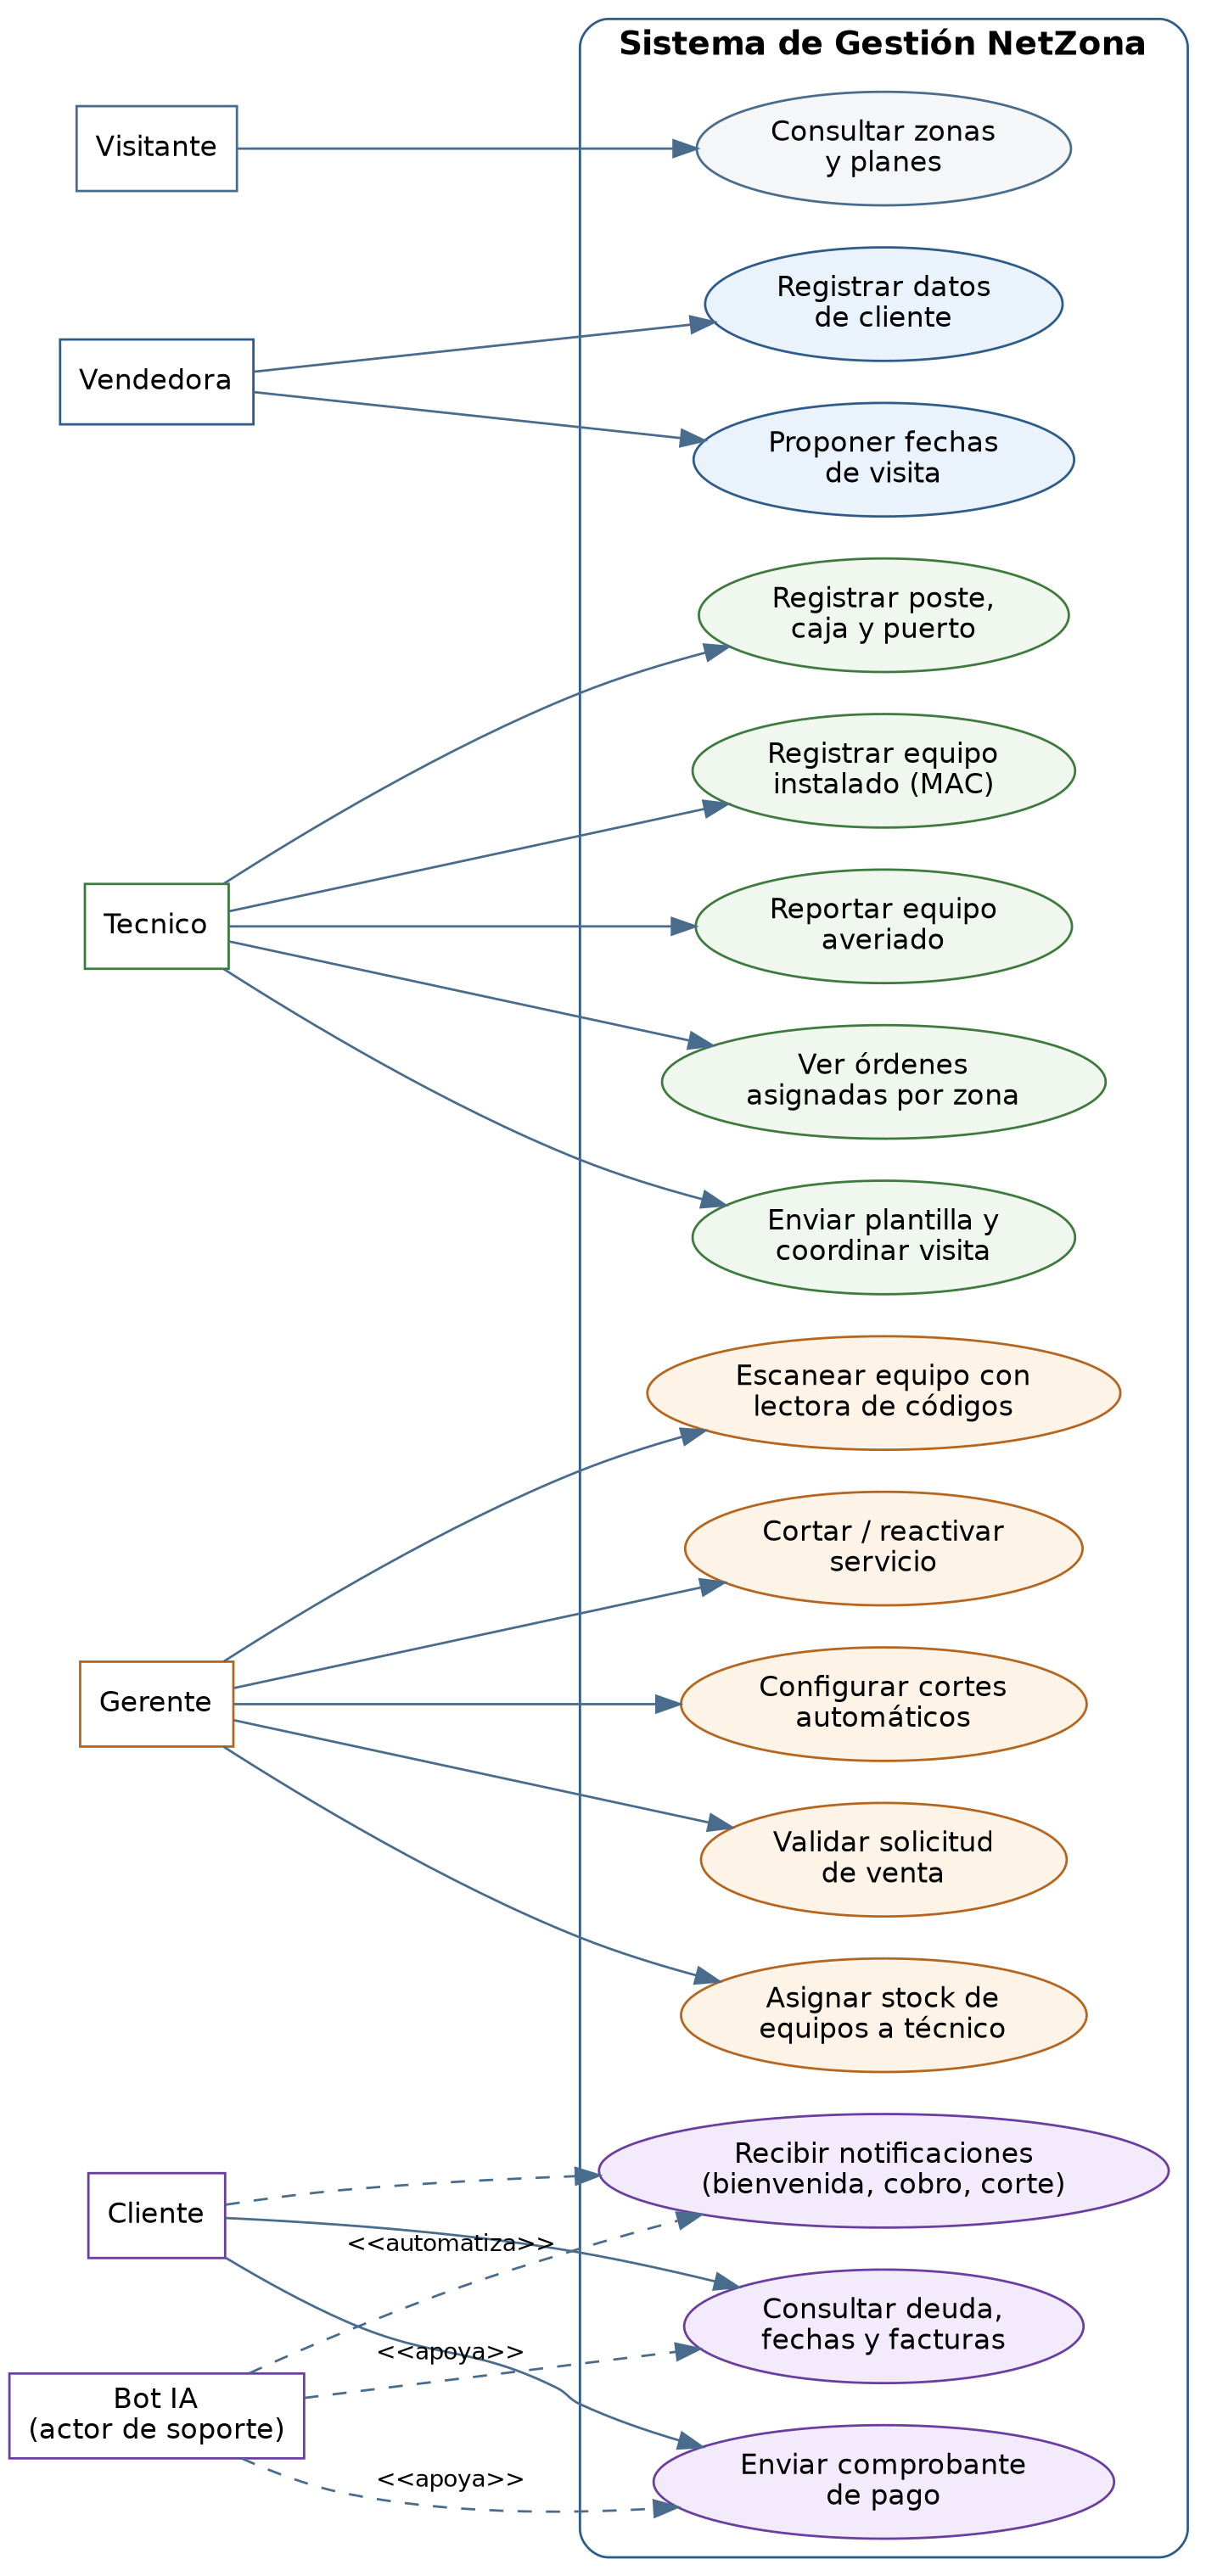
\includegraphics[width=\textwidth,height=0.45\textheight,keepaspectratio]{linea2/casos_uso.png}
\caption{Casos de uso del sistema por actor.}
\label{fig:ce02-casos-uso}
\end{figure}

% ======================================================================
\subsection{Modelo de dominio (diagrama de clases UML)}
\label{sec:ce02-clases}

El diagrama de clases de la \cref{fig:ce02-clases} es el \textbf{modelo de dominio
conceptual} elaborado en la fase de diseño: representa usuarios y roles, el flujo de
clientes y órdenes, la planta externa (postes, cajas NAP y puertos), el inventario de
equipos, los pagos y los mensajes, con sus relaciones y enumeraciones.

\begin{figure}[htbp]
\centering
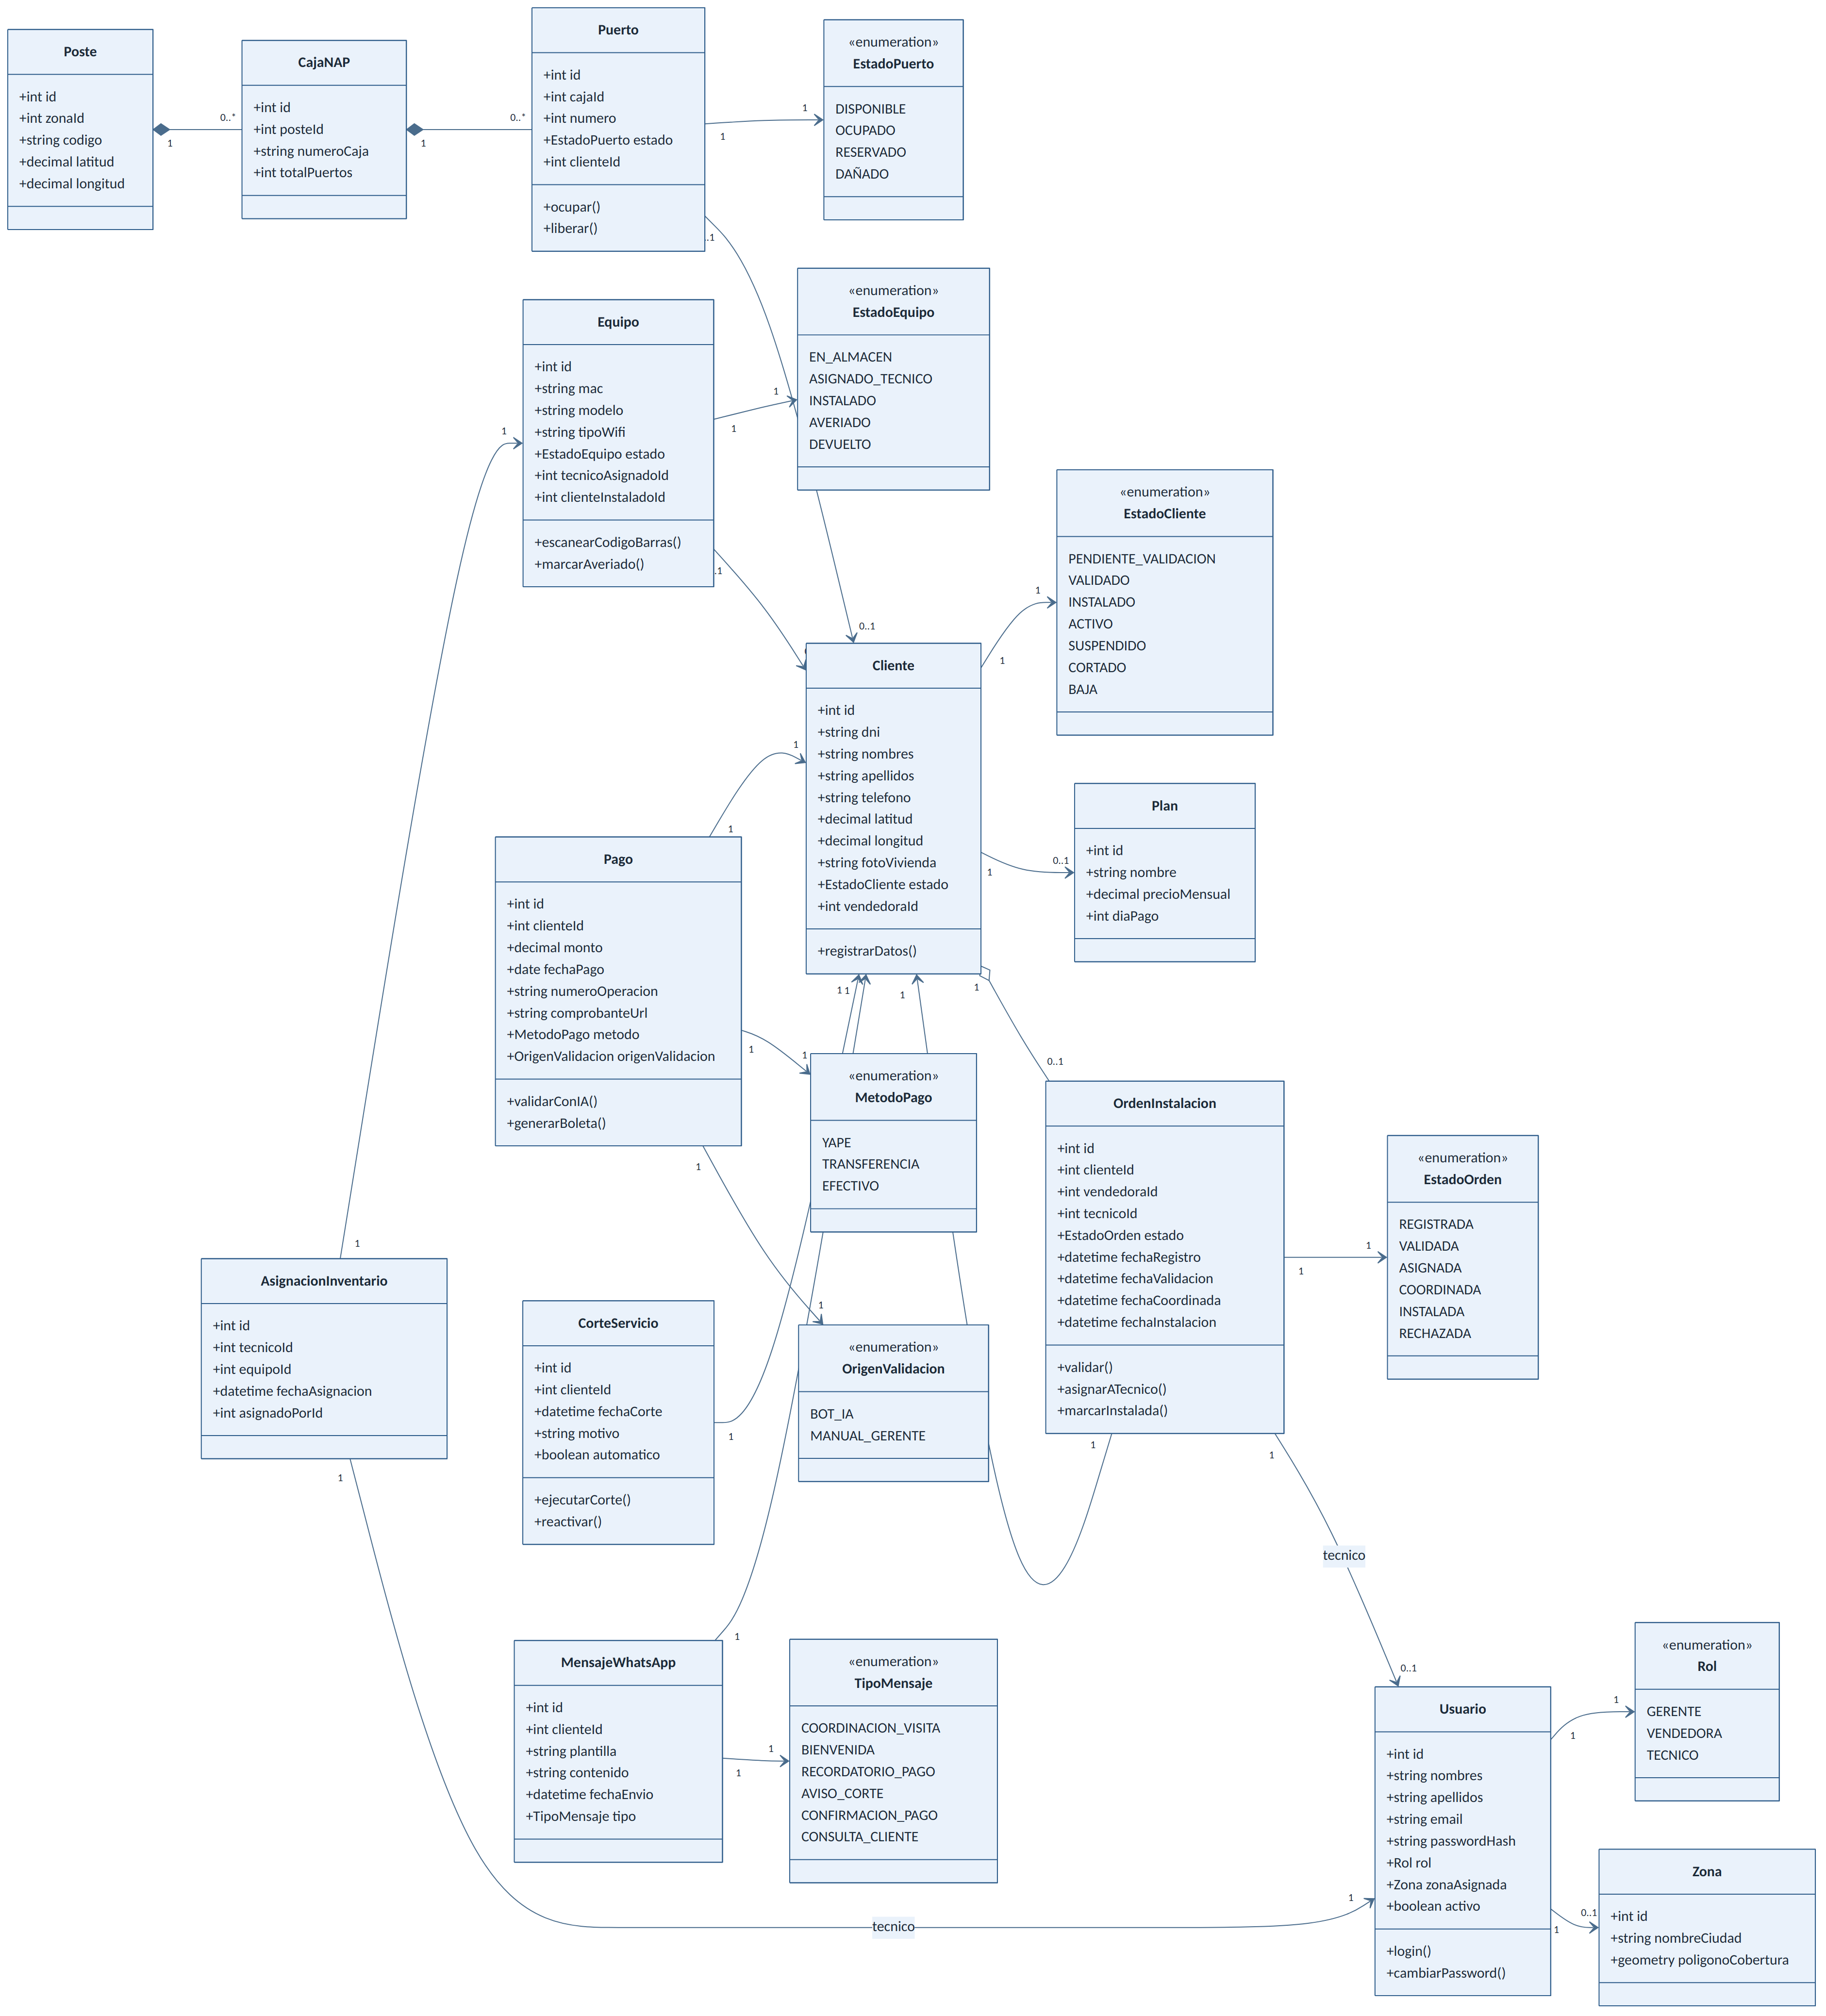
\includegraphics[width=\textwidth,height=0.62\textheight,keepaspectratio]{linea2/clases_dominio.png}
\caption{Modelo de dominio conceptual (diseño).}
\label{fig:ce02-clases}
\end{figure}

Durante la construcción, el modelo se refinó para reflejar el vocabulario real de la
planta de fibra y las necesidades descubiertas en la validación. La
\cref{tab:ce02-mapeo} documenta cada cambio, de modo que el diseño y la base de datos
(\cref{chap:ce02-datos}) sean trazables entre sí.

\begin{table}[htbp]
\centering
\caption{Refinamiento del modelo de dominio: diseño $\rightarrow$ implementación.}
\label{tab:ce02-mapeo}
\small
\begin{tabularx}{\textwidth}{L{3cm}L{3.4cm}X}
\toprule
\textbf{Clase de diseño} & \textbf{Entidad implementada} & \textbf{Motivo del cambio} \\
\midrule
Poste & \texttt{Mufa} + \texttt{Corrida} & En la planta real las cajas cuelgan de una mufa (empalme del troncal) y se unen por corridas de fibra con metraje; el poste no aporta información útil. \\
CajaNAP & \texttt{CajaNap} & Se agrega la mufa de origen y la capacidad de bornes (8 o 16). \\
Puerto & \texttt{Borne} & Término usado por los técnicos; se agregan precinto y potencia óptica (dBm). \\
Equipo & \texttt{Onu} & El equipo instalado es la ONU; se identifica por número de serie único. \\
OrdenInstalacion & Estados de \texttt{Cliente} & La orden no tenía datos propios: su ciclo se modela con los estados del cliente y los campos de aprobación e instalación. \\
CorteServicio & \texttt{Historial} (tipo \texttt{corte}) & Un corte es un evento del cliente; se registra en el historial con usuario y fecha. \\
MensajeWhatsApp & \texttt{MensajeMasivo} + \texttt{MensajeMasivoEnvio} & Se registra cada envío masivo y su resultado por destinatario. \\
AsignacionInventario & \texttt{Onu.tecnico\_id} + fecha & La asignación es un atributo de la ONU. \\
--- & \texttt{Averia}, \texttt{OrdenRetiro}, \texttt{Evidencia} & Operación de campo incorporada en la validación (RF-47, RF-48). \\
--- & \texttt{JornadaVendedor}, \texttt{UbicacionVendedor} & Recorrido del vendedor de campo (RF-49). \\
--- & \texttt{Gasto}, \texttt{ConsultaDocumentoMes} & Gastos por zona (RF-51) y control de cuota de la consulta DNI/RUC. \\
\bottomrule
\end{tabularx}
\end{table}

% ======================================================================
\subsection{Contratos de la API}
\label{sec:ce02-api}

La API está documentada automáticamente con OpenAPI (ruta \texttt{/docs}, oculta en
producción). Todas las rutas, salvo el login y la información pública, exigen un JWT
válido y un rol autorizado.

{\small
\begin{longtable}{L{1.2cm}L{5.2cm}L{2.4cm}L{5.0cm}}
\caption{Endpoints principales del sistema.}\label{tab:ce02-endpoints}\\
\toprule
\textbf{Método} & \textbf{Ruta} & \textbf{Rol} & \textbf{Función} \\
\midrule
\endfirsthead
\toprule
\textbf{Método} & \textbf{Ruta} & \textbf{Rol} & \textbf{Función} \\
\midrule
\endhead
\bottomrule
\endlastfoot
POST & \texttt{/api/auth/login} & Público & Devuelve el JWT (con freno a la fuerza bruta). \\
GET & \texttt{/api/zonas/publicas} & Público & Zonas con cobertura para el sitio web. \\
GET & \texttt{/api/clientes} & Interno & Lista paginada con filtros por zona y estado. \\
POST & \texttt{/api/clientes} & Admin, vendedor & Registra el cliente (estado inicial \texttt{pendiente\_aprobacion}). \\
POST & \texttt{/api/clientes/\{id\}/cortar} & Admin & Aviso por WhatsApp y corte en el MikroTik. \\
POST & \texttt{/api/clientes/\{id\}/reactivar} & Admin & Reactiva y extiende el vencimiento. \\
GET & \texttt{/api/clientes/\{id\}/pppoe-status} & Admin & Sesión PPPoE en tiempo real. \\
POST & \texttt{/api/pagos} & Admin, atención & Registra el pago, emite el recibo y reactiva si corresponde. \\
GET/POST & \texttt{/api/cajas-nap}, \texttt{/api/mufas} & Admin, técnico & Planta externa y bornes. \\
GET/POST & \texttt{/api/onus} & Admin, técnico & Inventario de ONU. \\
GET/POST & \texttt{/api/averias}, \texttt{/api/ordenes-retiro} & Admin, técnico & Operación de campo. \\
GET & \texttt{/api/zonas/\{id\}/wireguard-status} & Admin & Ping, SSH y \emph{handshake} del túnel. \\
POST & \texttt{/api/zonas/\{id\}/wireguard/peer} & Admin & Alta del peer en la VPS. \\
POST & \texttt{/api/zonas/\{id\}/exec} & Admin & Comando RouterOS restringido. \\
POST & \texttt{/api/whatsapp/broadcast-cobros} & Admin & Aviso masivo de cobro. \\
GET & \texttt{/api/cliente/me}, \texttt{/api/cliente/mis-pagos} & Cliente (PIN) & Autoservicio. \\
GET & \texttt{/api/health} & Público & Verificación de salud. \\
\end{longtable}
}

% ======================================================================
\subsection{Diagramas de secuencia}
\label{sec:ce02-secuencias}

Se modelan los cuatro flujos de interacción más importantes. Los diagramas
corresponden al diseño; las notas indican cómo quedó cada paso en la implementación.

\begin{figure}[htbp]
\centering
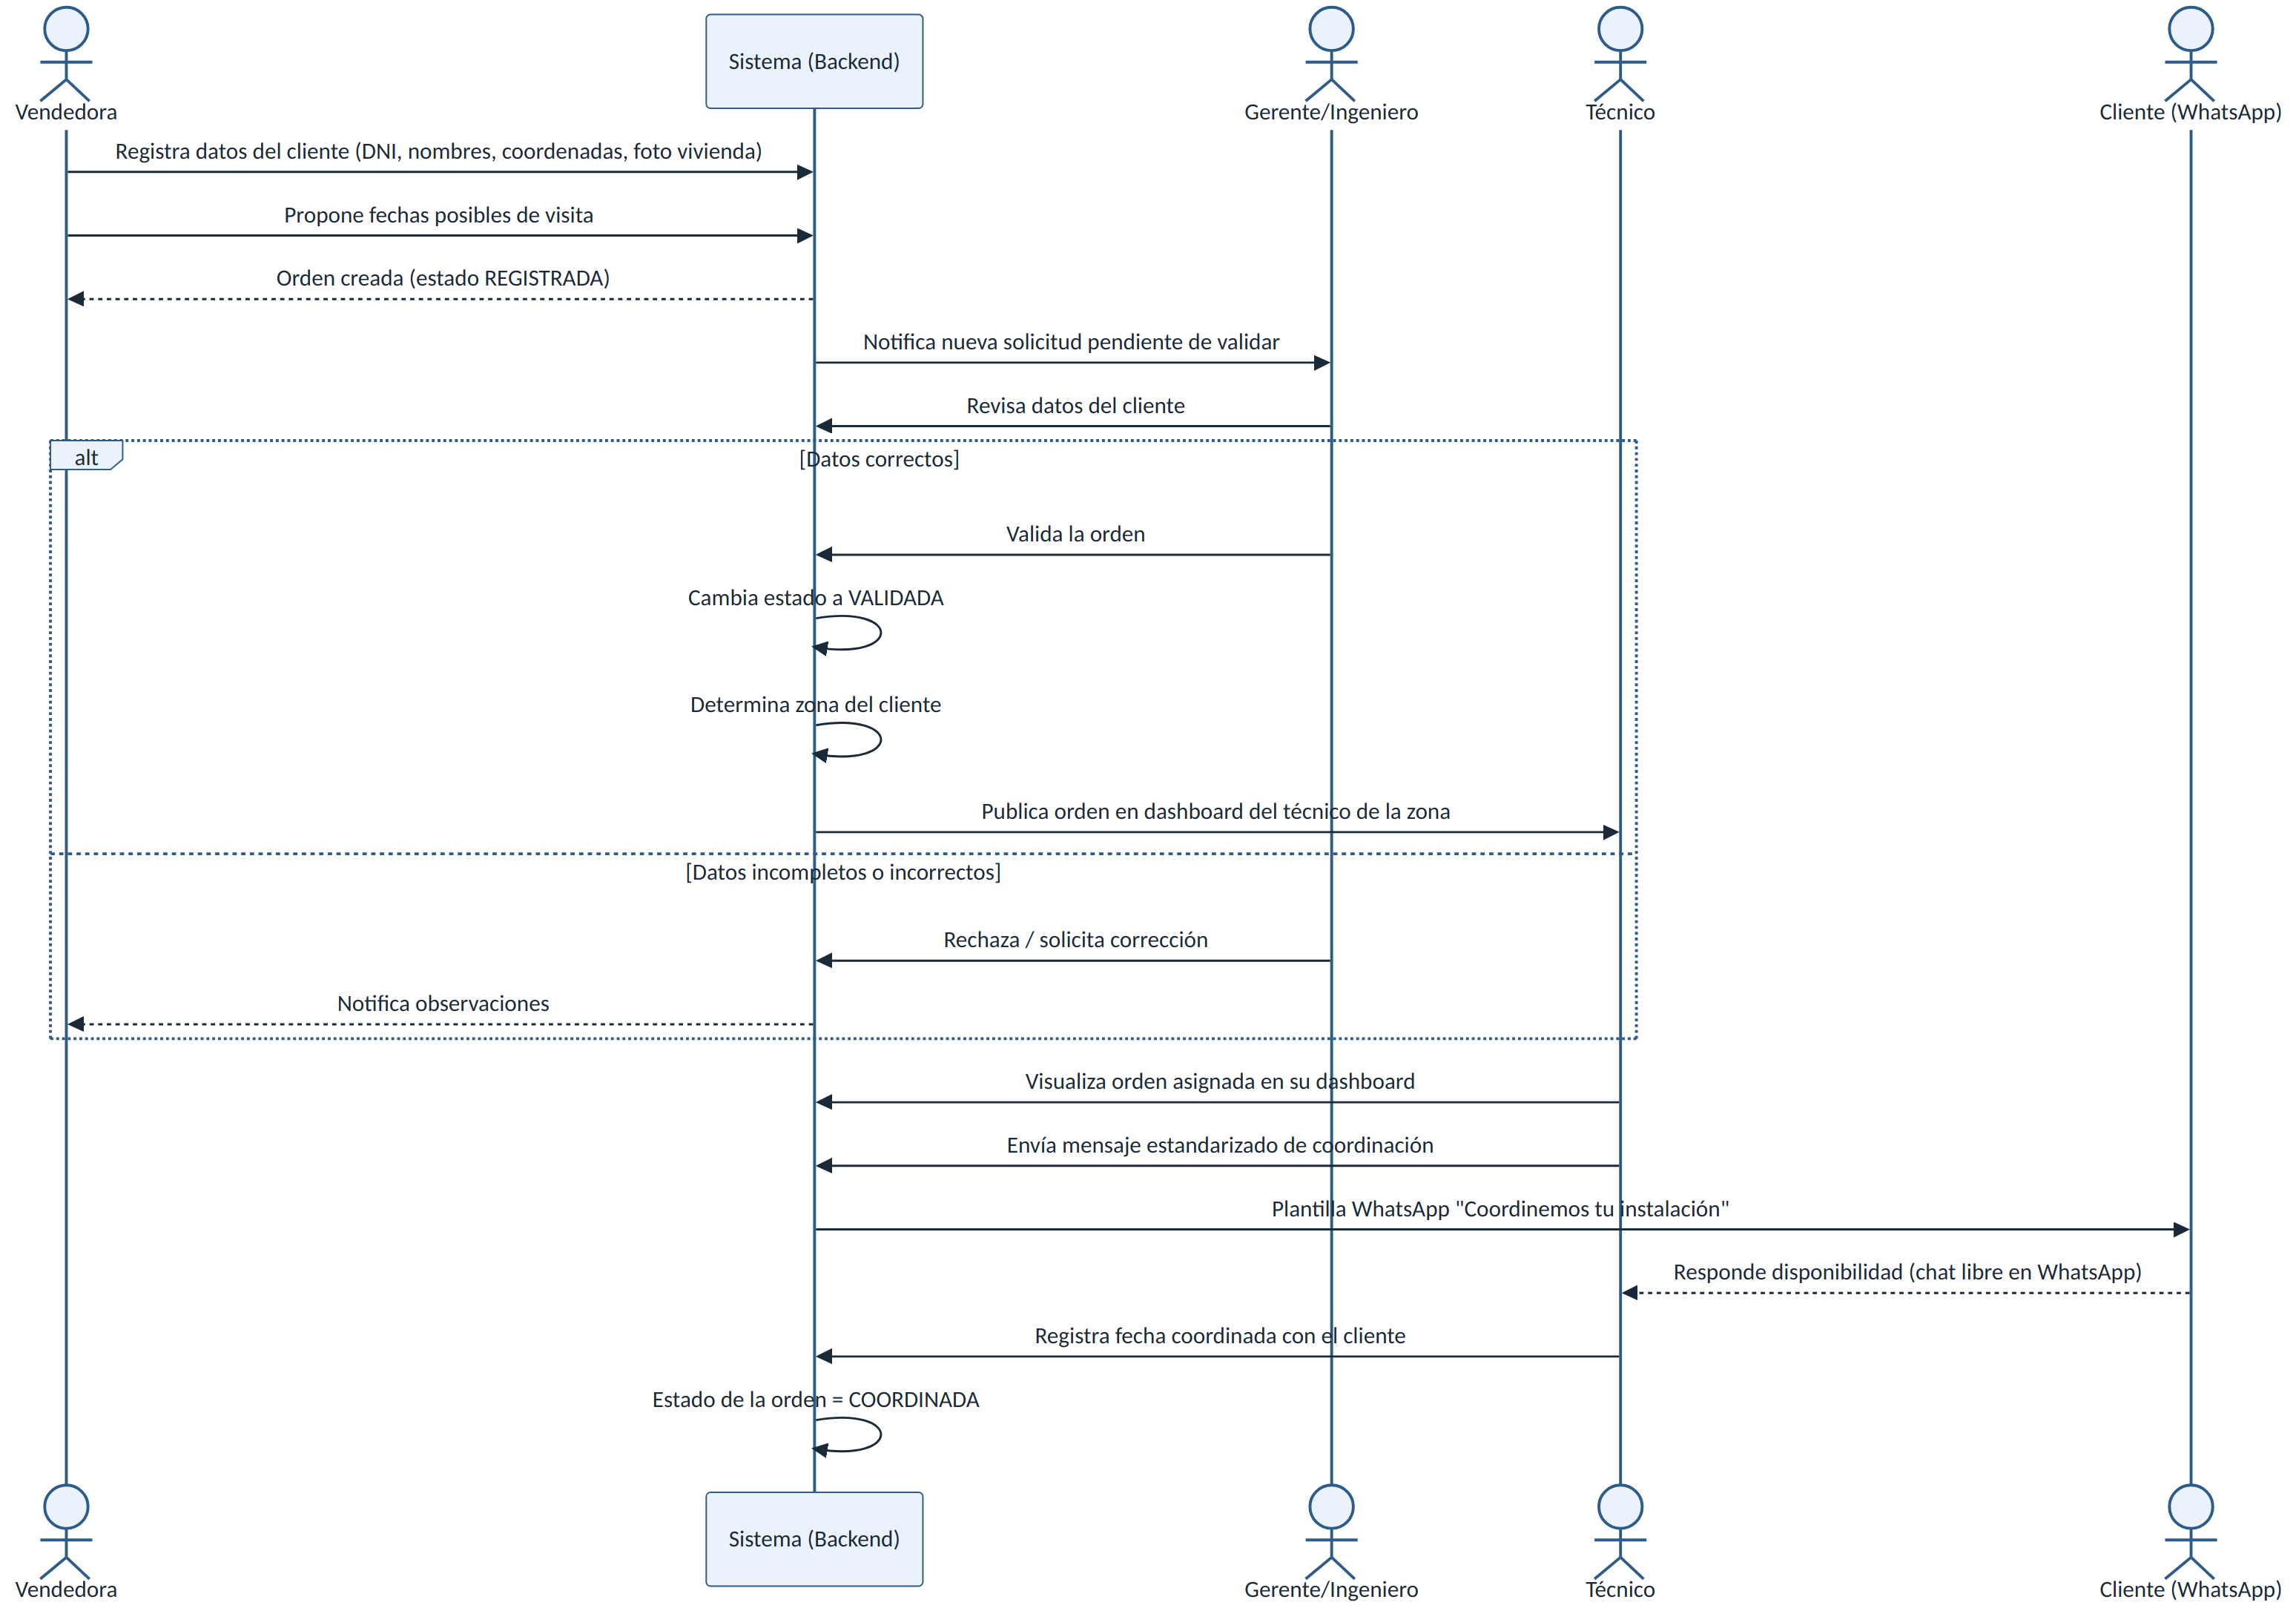
\includegraphics[width=\textwidth,height=0.4\textheight,keepaspectratio]{linea2/seq_venta.png}
\caption{Secuencia: registro de cliente, validación y coordinación de visita.}
\label{fig:ce02-seq-venta}
\end{figure}
\noindent\textit{Implementación:} registro y aprobación completos; el envío de la
plantilla de coordinación y la fecha acordada (RF-13, RF-14) están pendientes.

\begin{figure}[htbp]
\centering
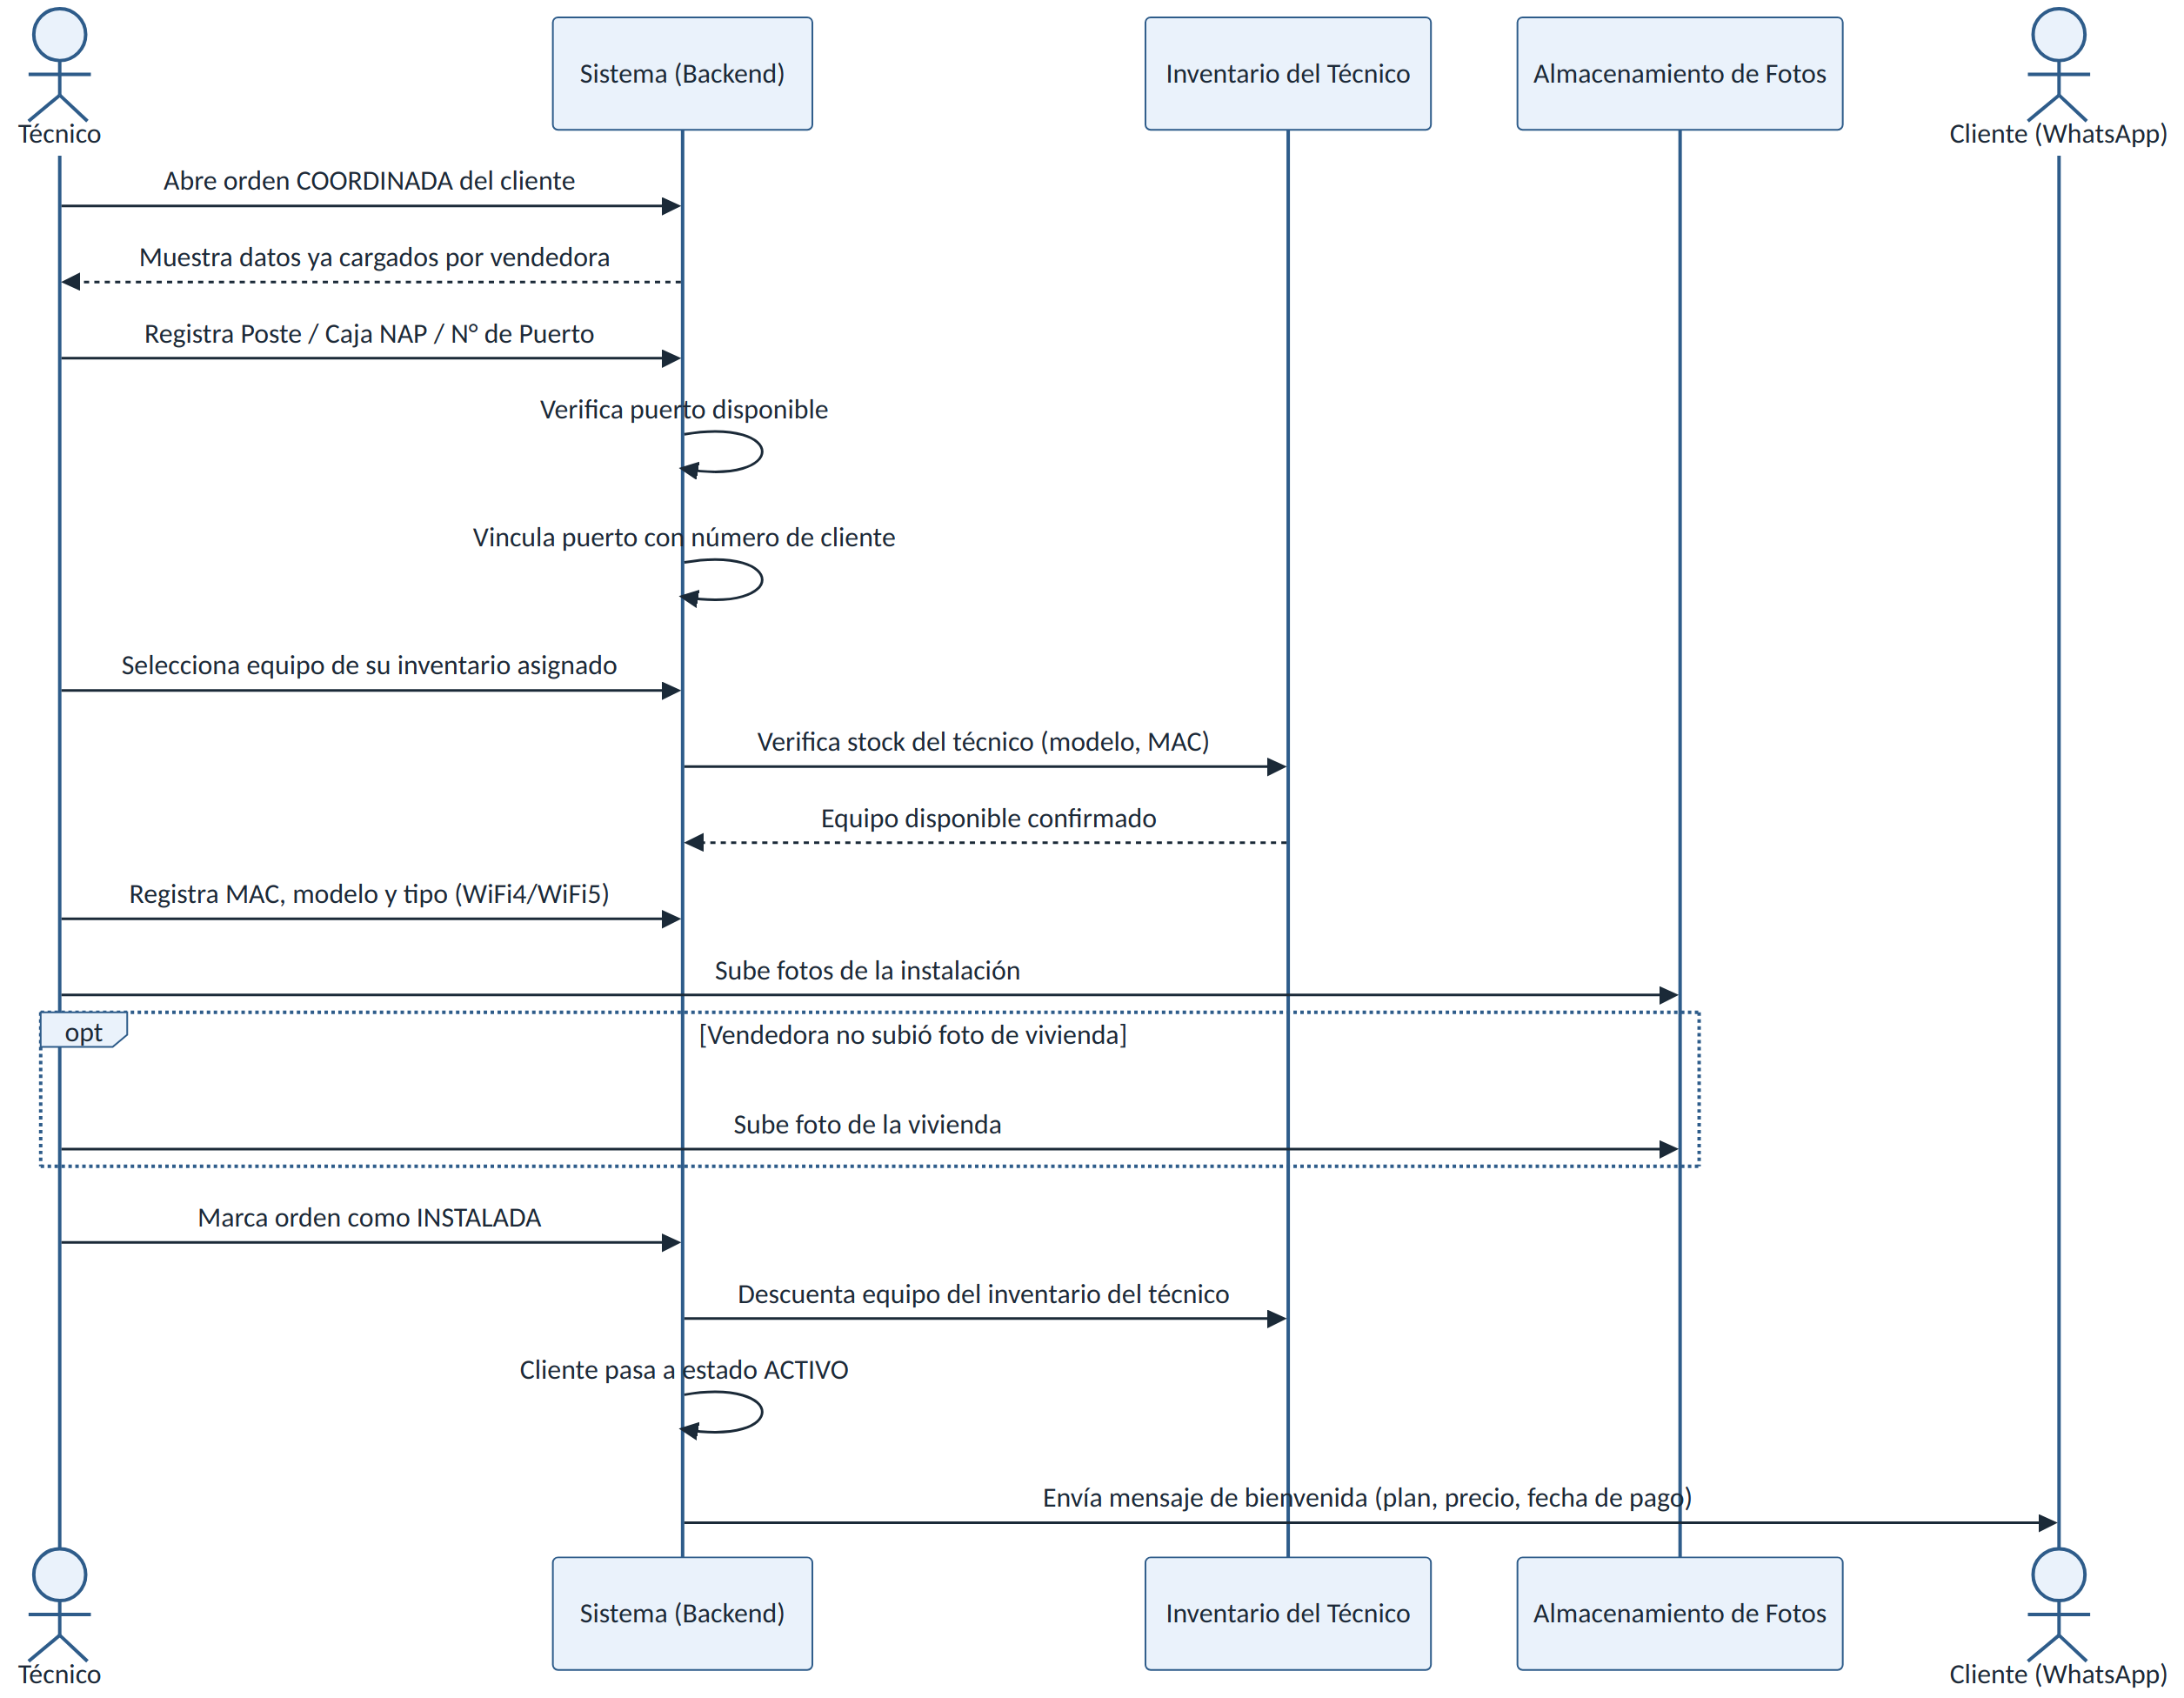
\includegraphics[width=\textwidth,height=0.4\textheight,keepaspectratio]{linea2/seq_instalacion.png}
\caption{Secuencia: registro de caja, borne, equipo y cierre de la instalación.}
\label{fig:ce02-seq-instalacion}
\end{figure}
\noindent\textit{Implementación:} al cerrar, el backend crea el secreto PPPoE en el
MikroTik de la zona por SSH, marca el borne como ocupado y la ONU como instalada, y
activa al cliente.

\begin{figure}[htbp]
\centering
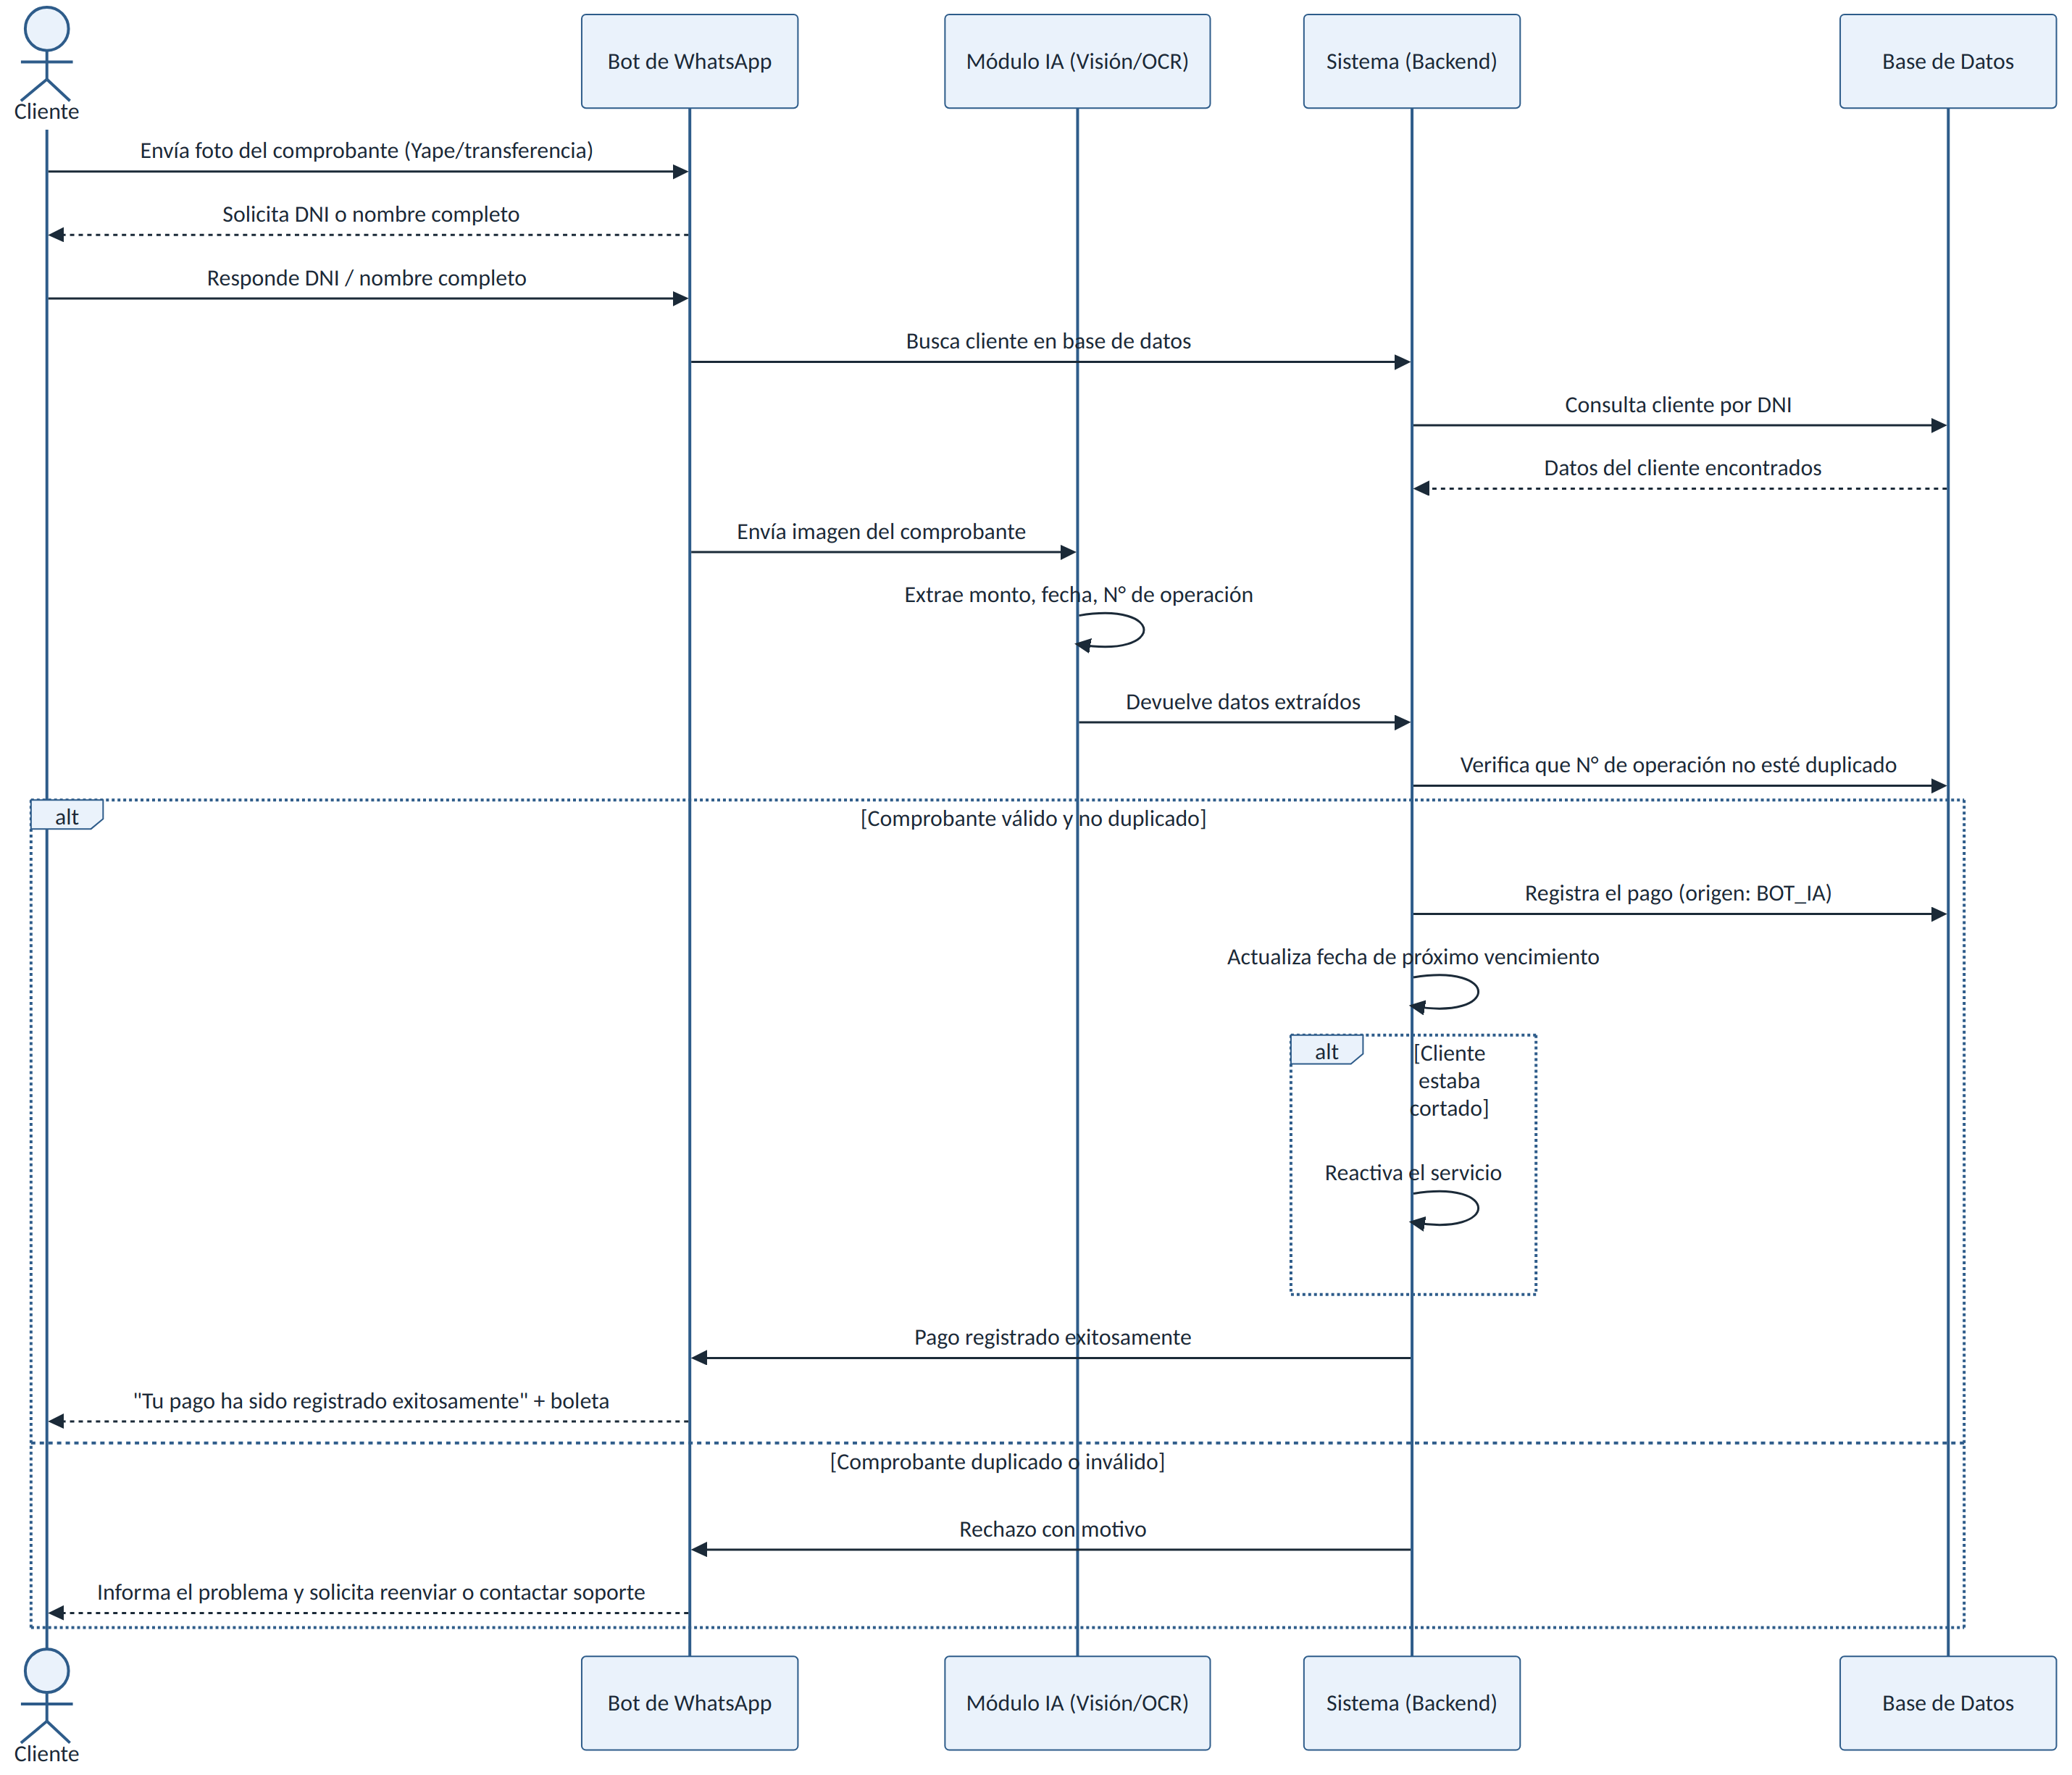
\includegraphics[width=\textwidth,height=0.4\textheight,keepaspectratio]{linea2/seq_pago.png}
\caption{Secuencia (diseño): validación de pago con IA por WhatsApp.}
\label{fig:ce02-seq-pago}
\end{figure}
\noindent\textit{Implementación:} diferida (ADR-06). Hoy el pago lo registra el
personal; la base de datos rechaza números de operación repetidos.

\begin{figure}[htbp]
\centering
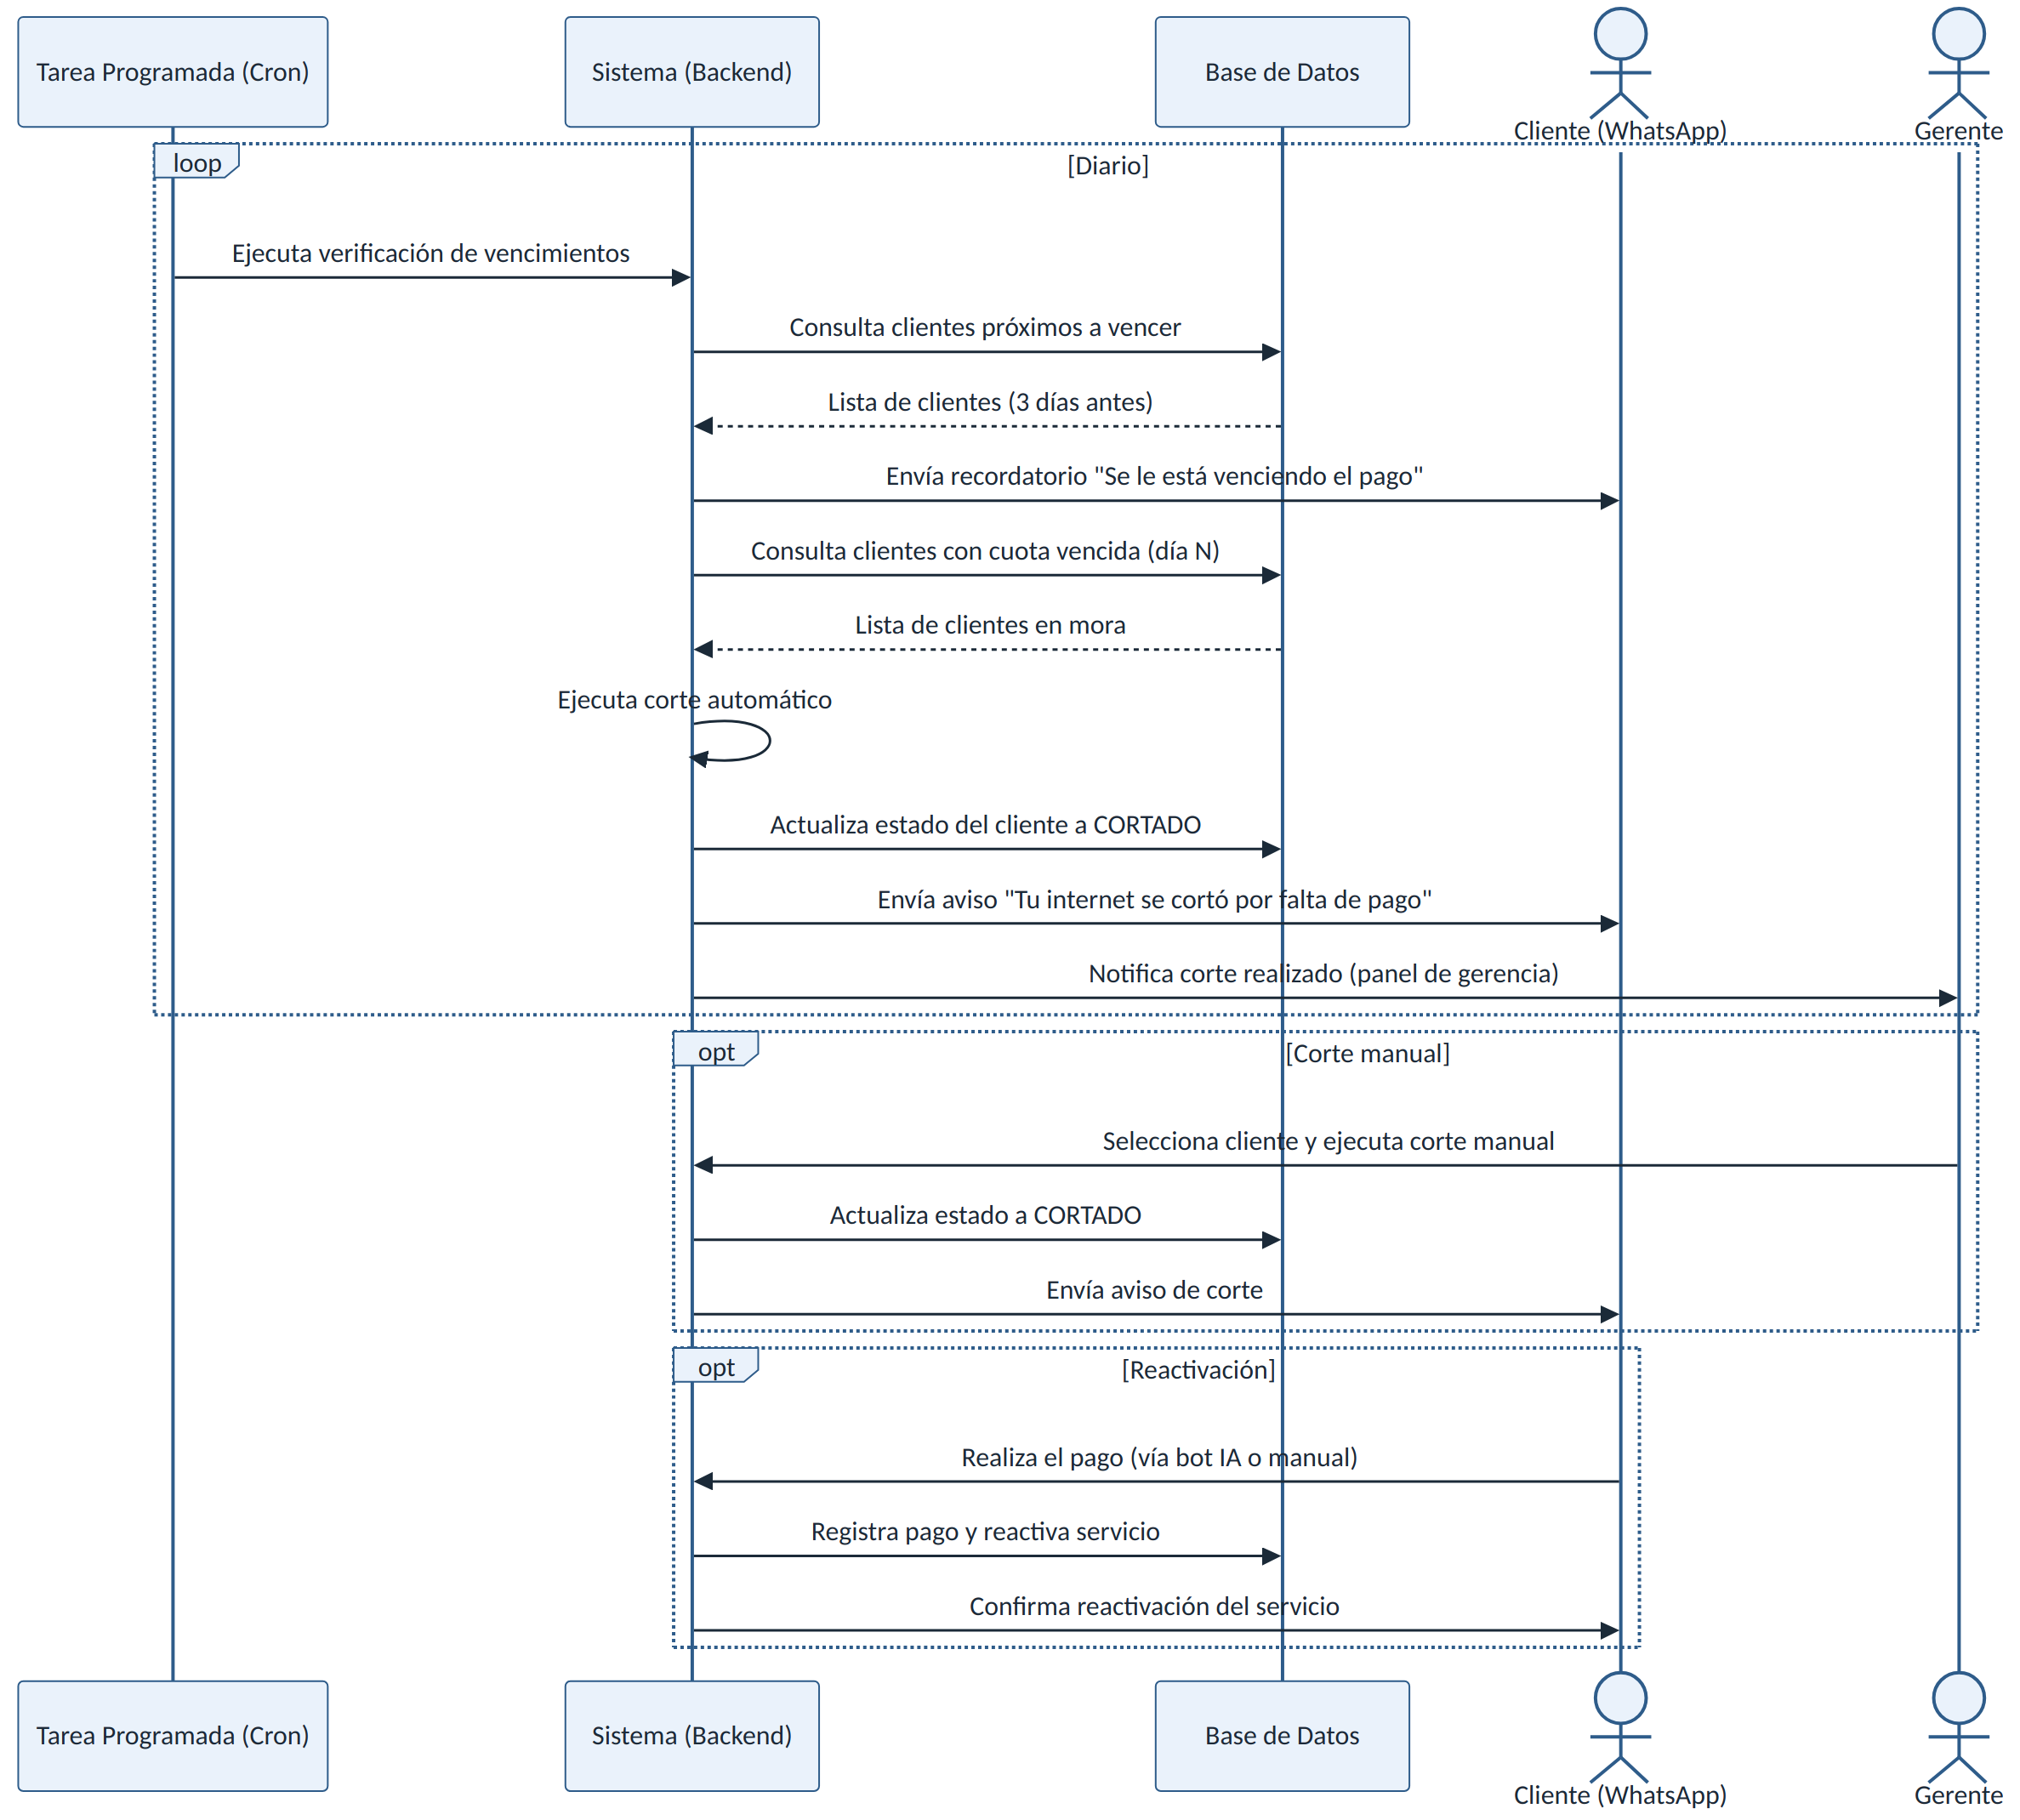
\includegraphics[width=\textwidth,height=0.4\textheight,keepaspectratio]{linea2/seq_corte.png}
\caption{Secuencia: recordatorio, corte automático o manual y reactivación.}
\label{fig:ce02-seq-corte}
\end{figure}
\noindent\textit{Implementación:} el aviso se envía antes del corte (RN-09); el corte
agrega la IP del cliente a la lista de corte configurada para su zona.

% ======================================================================
\subsection{Diagramas de estados}
\label{sec:ce02-estados}

Los diagramas siguientes reflejan los estados reales definidos en
\texttt{backend/app/models.py}.

\tikzset{estado/.style={draw=upeublue,fill=upeublue!8,rounded corners=6pt,font=\scriptsize,
  minimum width=2.3cm,minimum height=7mm,align=center},
  ini/.style={circle,fill=upeublue,minimum size=3mm,inner sep=0pt},
  trans/.style={-{Stealth[length=2mm]},draw=upeublue!80,thick},
  et/.style={font=\tiny,fill=white,inner sep=1pt}}

\begin{figure}[htbp]
\centering
\begin{tikzpicture}[node distance=11mm and 15mm]
  \node[ini] (i) {};
  \node[estado,right=8mm of i] (pend) {pendiente\_aprobacion};
  \node[estado,right=of pend] (apr) {aprobado};
  \node[estado,above=of apr] (rech) {rechazado};
  \node[estado,right=of apr] (act) {activo};
  \node[estado,below=of apr] (noi) {no\_instalado};
  \node[estado,above=of act] (pau) {pausado};
  \node[estado,below=of act] (sus) {suspendido};
  \node[estado,right=14mm of sus] (anu) {anulado};
  \draw[trans] (i) -- (pend);
  \draw[trans] (pend) -- node[et,above]{admin aprueba} (apr);
  \draw[trans] (pend) |- node[et,pos=0.7,above]{admin rechaza} (rech);
  \draw[trans] (apr) -- node[et,above]{instalación cerrada} (act);
  \draw[trans] (apr) -- node[et,left]{no se pudo instalar} (noi);
  \draw[trans] (act.150) -- node[et,left]{pausa} (pau.210);
  \draw[trans] (pau.330) -- node[et,right]{fin de pausa} (act.30);
  \draw[trans] (act.210) -- node[et,left]{corte (mora)} (sus.150);
  \draw[trans] (sus.30) -- node[et,right]{pago / reactivación} (act.330);
  \draw[trans] (sus) -- node[et,below]{baja / retiro} (anu);
  \draw[trans] (act.east) -| node[et,pos=0.3,above]{baja} (anu.north);
\end{tikzpicture}
\caption{Ciclo de vida del cliente (\texttt{EstadoCliente}). Cubre también la antigua
\emph{orden de instalación}.}
\label{fig:ce02-est-cliente}
\end{figure}

\begin{figure}[htbp]
\centering
\begin{tikzpicture}[node distance=9mm and 16mm]
  \node[ini] (i) {};
  \node[estado,right=of i] (alm) {en\_almacen};
  \node[estado,right=of alm] (asg) {asignado\_tecnico};
  \node[estado,right=of asg] (ins) {instalado};
  \node[estado,below=of asg] (dan) {danado};
  \node[estado,above=of asg] (per) {perdido};
  \draw[trans] (i) -- node[et,above]{registro (escaneo)} (alm);
  \draw[trans] (alm) -- node[et,above]{asignar a técnico} (asg);
  \draw[trans] (asg) -- node[et,above]{instalación} (ins);
  \draw[trans] (ins.south) |- node[et,pos=0.25,right]{avería: reemplazo} (dan.east);
  \draw[trans] (asg) -- node[et,right]{reporte de daño} (dan);
  \draw[trans] (asg) -- node[et,right]{extravío} (per);
  \draw[trans] (ins.north) to[out=120,in=60] node[et,above]{retiro en buen estado} (alm.north);
\end{tikzpicture}
\caption{Ciclo de vida de la ONU (\texttt{EstadoOnu}).}
\label{fig:ce02-est-onu}

\vspace{8mm}
\begin{tikzpicture}[node distance=14mm]
  \node[ini] (i) {};
  \node[estado,right=of i] (p) {pendiente};
  \node[estado,right=of p] (a) {asignada};
  \node[estado,right=of a] (e) {en\_proceso};
  \node[estado,right=of e] (r) {resuelta};
  \draw[trans] (i) -- (p);
  \draw[trans] (p) -- node[et,above]{asignar técnico} (a);
  \draw[trans] (a) -- node[et,above]{inicia atención} (e);
  \draw[trans] (e) -- node[et,above]{diagnóstico + fotos} (r);
\end{tikzpicture}
\caption{Ciclo de vida de una avería (\texttt{EstadoAveria}).}
\label{fig:ce02-est-averia}
\end{figure}

El estado de cada borne (\texttt{libre}, \texttt{ocupado}, \texttt{danado}) y de cada
pago (\texttt{pagado}, \texttt{pendiente}, \texttt{vencido}, \texttt{corte\_temporal})
completa el modelo de comportamiento; sus reglas se describen en la
\cref{sec:ce02-rn}.
